\documentclass[landscape,final,a0paper,fontscale=0.285]{baposter}

\usepackage{calc}
\usepackage{graphicx}
\usepackage{amsmath}
\usepackage{amssymb}
\usepackage{relsize}
\usepackage{multirow}
\usepackage{rotating}
\usepackage{bm}
\usepackage{url}

\usepackage{graphicx}
\usepackage{multicol}

%\usepackage{times}
%\usepackage{helvet}
%\usepackage{bookman}
\usepackage{palatino}

\newcommand{\captionfont}{\footnotesize}

\graphicspath{{images/}{../images/}}
\usetikzlibrary{calc}

\newcommand{\SET}[1]  {\ensuremath{\mathcal{#1}}}
\newcommand{\MAT}[1]  {\ensuremath{\boldsymbol{#1}}}
\newcommand{\VEC}[1]  {\ensuremath{\boldsymbol{#1}}}
\newcommand{\Video}{\SET{V}}
\newcommand{\video}{\VEC{f}}
\newcommand{\track}{x}
\newcommand{\Track}{\SET T}
\newcommand{\LMs}{\SET L}
\newcommand{\lm}{l}
\newcommand{\PosE}{\SET P}
\newcommand{\posE}{\VEC p}
\newcommand{\negE}{\VEC n}
\newcommand{\NegE}{\SET N}
\newcommand{\Occluded}{\SET O}
\newcommand{\occluded}{o}

%%%%%%%%%%%%%%%%%%%%%%%%%%%%%%%%%%%%%%%%%%%%%%%%%%%%%%%%%%%%%%%%%%%%%%%%%%%%%%%%
%%%% Some math symbols used in the text
%%%%%%%%%%%%%%%%%%%%%%%%%%%%%%%%%%%%%%%%%%%%%%%%%%%%%%%%%%%%%%%%%%%%%%%%%%%%%%%%

%%%%%%%%%%%%%%%%%%%%%%%%%%%%%%%%%%%%%%%%%%%%%%%%%%%%%%%%%%%%%%%%%%%%%%%%%%%%%%%%
% Multicol Settings
%%%%%%%%%%%%%%%%%%%%%%%%%%%%%%%%%%%%%%%%%%%%%%%%%%%%%%%%%%%%%%%%%%%%%%%%%%%%%%%%
\setlength{\columnsep}{1.5em}
\setlength{\columnseprule}{0mm}

%%%%%%%%%%%%%%%%%%%%%%%%%%%%%%%%%%%%%%%%%%%%%%%%%%%%%%%%%%%%%%%%%%%%%%%%%%%%%%%%
% Save space in lists. Use this after the opening of the list
%%%%%%%%%%%%%%%%%%%%%%%%%%%%%%%%%%%%%%%%%%%%%%%%%%%%%%%%%%%%%%%%%%%%%%%%%%%%%%%%
\newcommand{\compresslist}{%
\setlength{\itemsep}{1pt}%
\setlength{\parskip}{0pt}%
\setlength{\parsep}{0pt}%
}

%%%%%%%%%%%%%%%%%%%%%%%%%%%%%%%%%%%%%%%%%%%%%%%%%%%%%%%%%%%%%%%%%%%%%%%%%%%%%%
%%% Begin of Document
%%%%%%%%%%%%%%%%%%%%%%%%%%%%%%%%%%%%%%%%%%%%%%%%%%%%%%%%%%%%%%%%%%%%%%%%%%%%%%

\begin{document}

%%%%%%%%%%%%%%%%%%%%%%%%%%%%%%%%%%%%%%%%%%%%%%%%%%%%%%%%%%%%%%%%%%%%%%%%%%%%%%
%%% Here starts the poster
%%%---------------------------------------------------------------------------
%%% Format it to your taste with the options
%%%%%%%%%%%%%%%%%%%%%%%%%%%%%%%%%%%%%%%%%%%%%%%%%%%%%%%%%%%%%%%%%%%%%%%%%%%%%%
% Define some colors

%\definecolor{lightblue}{cmyk}{0.83,0.24,0,0.12}
\definecolor{lightblue}{rgb}{0.05,0.66,1}
\definecolor{mblue}{rgb}{0.0,0.33,0.9}

% Draw a video
\newlength{\FSZ}
\newcommand{\drawvideo}[3]{% [0 0.25 0.5 0.75 1 1.25 1.5]
   \noindent\pgfmathsetlength{\FSZ}{\linewidth/#2}
   \begin{tikzpicture}[outer sep=0pt,inner sep=0pt,x=\FSZ,y=\FSZ]
   \draw[color=lightblue!50!black] (0,0) node[outer sep=0pt,inner sep=0pt,text width=\linewidth,minimum height=0] (video) {\noindent#3};
   \path [fill=lightblue!50!black,line width=0pt] 
     (video.north west) rectangle ([yshift=\FSZ] video.north east) 
    \foreach \x in {1,2,...,#2} {
      {[rounded corners=0.6] ($(video.north west)+(-0.7,0.8)+(\x,0)$) rectangle +(0.4,-0.6)}
    }
;
   \path [fill=lightblue!50!black,line width=0pt] 
     ([yshift=-1\FSZ] video.south west) rectangle (video.south east) 
    \foreach \x in {1,2,...,#2} {
      {[rounded corners=0.6] ($(video.south west)+(-0.7,-0.2)+(\x,0)$) rectangle +(0.4,-0.6)}
    }
;
   \foreach \x in {1,...,#1} {
     \draw[color=lightblue!50!black] ([xshift=\x\linewidth/#1] video.north west) -- ([xshift=\x\linewidth/#1] video.south west);
   }
   \foreach \x in {0,#1} {
     \draw[color=lightblue!50!black] ([xshift=\x\linewidth/#1,yshift=1\FSZ] video.north west) -- ([xshift=\x\linewidth/#1,yshift=-1\FSZ] video.south west);
   }
   \end{tikzpicture}
}

\hyphenation{resolution occlusions}
%%
\begin{poster}%
  % Poster Options
  {
  % Show grid to help with alignment
  grid=false,
  % Column spacing
  colspacing=1em,
  % Color style
  bgColorOne=white,
  bgColorTwo=white,
  borderColor=lightblue,
  headerColorOne=mblue,
  headerColorTwo=lightblue,
  headerFontColor=white,
  boxColorOne=white,
  boxColorTwo=lightblue,
  % Format of textbox
  %textborder=roundedleft,
  % Format of text header
  eyecatcher=false,
  headerborder=closed,
  headerheight=0.1\textheight,
%  textfont=\sc, An example of changing the text font
  %headershape=roundedright,
  headershade=shadelr,
  headerfont=\Large\bf\textsc, %Sans Serif
  textfont={\setlength{\parindent}{1.5em}},
  boxshade=plain,
%  background=shade-tb,
  background=plain,
  linewidth=1pt
  }
  % U Logo
  {
\includegraphics[height=5em]{../images/ubourgogne}} 
  % Title
  {\bf\textsc{Object Flow: A per-object dense motion descriptor}\vspace{0.5em}}
  % Authors
  {\textsc{Juan M. Perez Rua, Tomas Crivelli and Patrick Perez}}
  % Technicolor logo
  {% The makebox allows the title to flow into the logo, this is a hack because of the L shaped logo.
    
\includegraphics[height=6.6em]{../images/technicolor_large}
  }

%%%%%%%%%%%%%%%%%%%%%%%%%%%%%%%%%%%%%%%%%%%%%%%%%%%%%%%%%%%%%%%%%%%%%%%%%%%%%%
%%% Now define the boxes that make up the poster
%%%---------------------------------------------------------------------------
%%% Each box has a name and can be placed absolutely or relatively.
%%% The only inconvenience is that you can only specify a relative position 
%%% towards an already declared box. So if you have a box attached to the 
%%% bottom, one to the top and a third one which should be in between, you 
%%% have to specify the top and bottom boxes before you specify the middle 
%%% box.
%%%%%%%%%%%%%%%%%%%%%%%%%%%%%%%%%%%%%%%%%%%%%%%%%%%%%%%%%%%%%%%%%%%%%%%%%%%%%%
    %
    % A coloured circle useful as a bullet with an adjustably strong filling
    \newcommand{\colouredcircle}{%
      \tikz{\useasboundingbox (-0.2em,-0.32em) rectangle(0.2em,0.32em); \draw[draw=black,fill=lightblue,line width=0.03em] (0,0) circle(0.18em);}}

%%%%%%%%%%%%%%%%%%%%%%%%%%%%%%%%%%%%%%%%%%%%%%%%%%%%%%%%%%%%%%%%%%%%%%%%%%%%%%
  \headerbox{1. Definition}{name=definition,column=0,row=0}{
%%%%%%%%%%%%%%%%%%%%%%%%%%%%%%%%%%%%%%%%%%%%%%%%%%%%%%%%%%%%%%%%%%%%%%%%%%%%%%
	
Given a video sequence $I_t, t:0..N-1$, and an initial bounding box loosely indicating the position of an object in $I_0$.
 Let $\mathcal{R} \in \Omega$ be the region corresponding to the support of the object in the
bi-dimensional grid $\Omega$. Then, \textbf{ the object flow}, $\mathcal{O}(x)$,  is defined as $\mathcal{O}(x) = d_{0,t}(x), \forall x \in \mathcal{R}$.
With $d_{0,t}(x)$ a displacement vector between the frame $0$ and the frame $t$ for the pixel $x$.

      \centering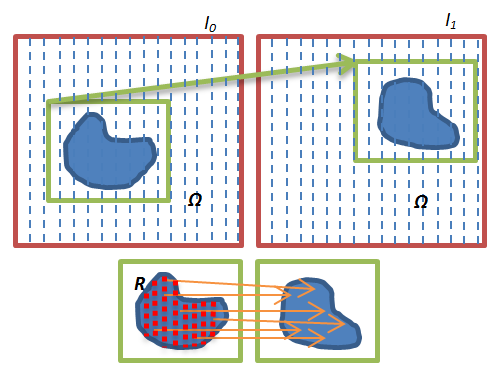
\includegraphics[width=1.0\textwidth]{../images/diagram.png}

 }

%%%%%%%%%%%%%%%%%%%%%%%%%%%%%%%%%%%%%%%%%%%%%%%%%%%%%%%%%%%%%%%%%%%%%%%%%%%%%%
  \headerbox{3. Background Tracking}{name=bgtrack,column=1,row=0,bottomaligned=definition}{
%%%%%%%%%%%%%%%%%%%%%%%%%%%%%%%%%%%%%%%%%%%%%%%%%%%%%%%%%%%%%%%%%%%%%%%%%%%%%%
     \centering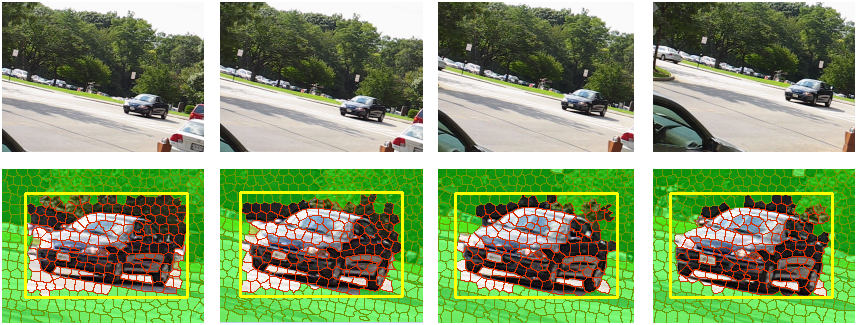
\includegraphics[width=1.0\textwidth]{../images/suppixflow2.png}
     \raggedright Obvious background superpixels (Outside tracking window) are labeled and tracked with the 
\textbf{ superpixel flow}. The superpixel flow is an energy based matching method for superpixels:

     \vspace{1.5 mm}

     \centering
     $ E(l) = \displaystyle \sum_{p \in \Gamma} D_p(l_p;I_0,I_1) +
     \sum_{(p,q): q \in \mathcal{N}_r} S_{p,q}(l_p,l_q), $ \\
     \raggedright with,  $ D_p(l_p;I_0,I_1) = \rho (\boldsymbol{h}(p), \boldsymbol{h}(p')) $, \\
     and,  $ S_{p,q}(l_p, l_q) = \lambda(p)
  \sqrt{\frac{|u_{p_c}-u_{q_c}|}{\|p_c-q_c\|}+ \frac{|v_{p_c}-v_{q_c}|}{\|p_c-q_c\|}}. $ \\

     \vspace{1.5 mm}

    The mask is finally refined with \cite{c3}.
    \centerline{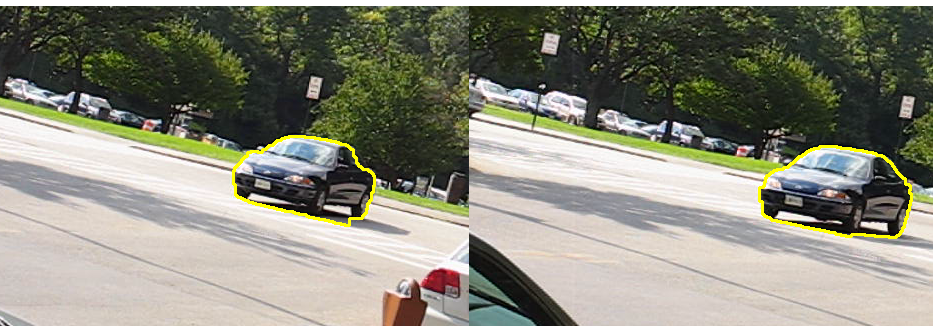
\includegraphics[width=0.8\textwidth]{../images/carSeg.png}}
}

%%%%%%%%%%%%%%%%%%%%%%%%%%%%%%%%%%%%%%%%%%%%%%%%%%%%%%%%%%%%%%%%%%%%%%%%%%%%%%
\headerbox{5. Results}{name=results,column=2,span=2,row=0}{
The object flows captures the motion details much better than globally computed optical flow methods.
\vfill
  \centering
  \begin{tabular}{cc}
  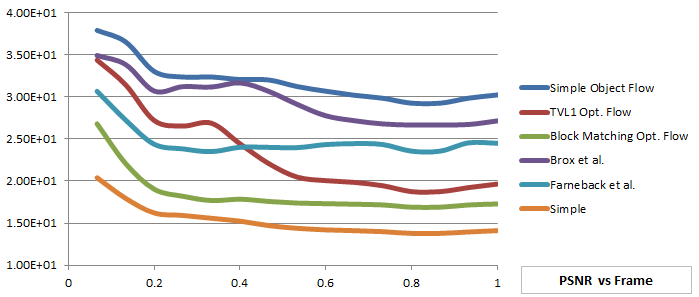
\includegraphics[width=0.5\textwidth]{../images/psnr2.png}&
  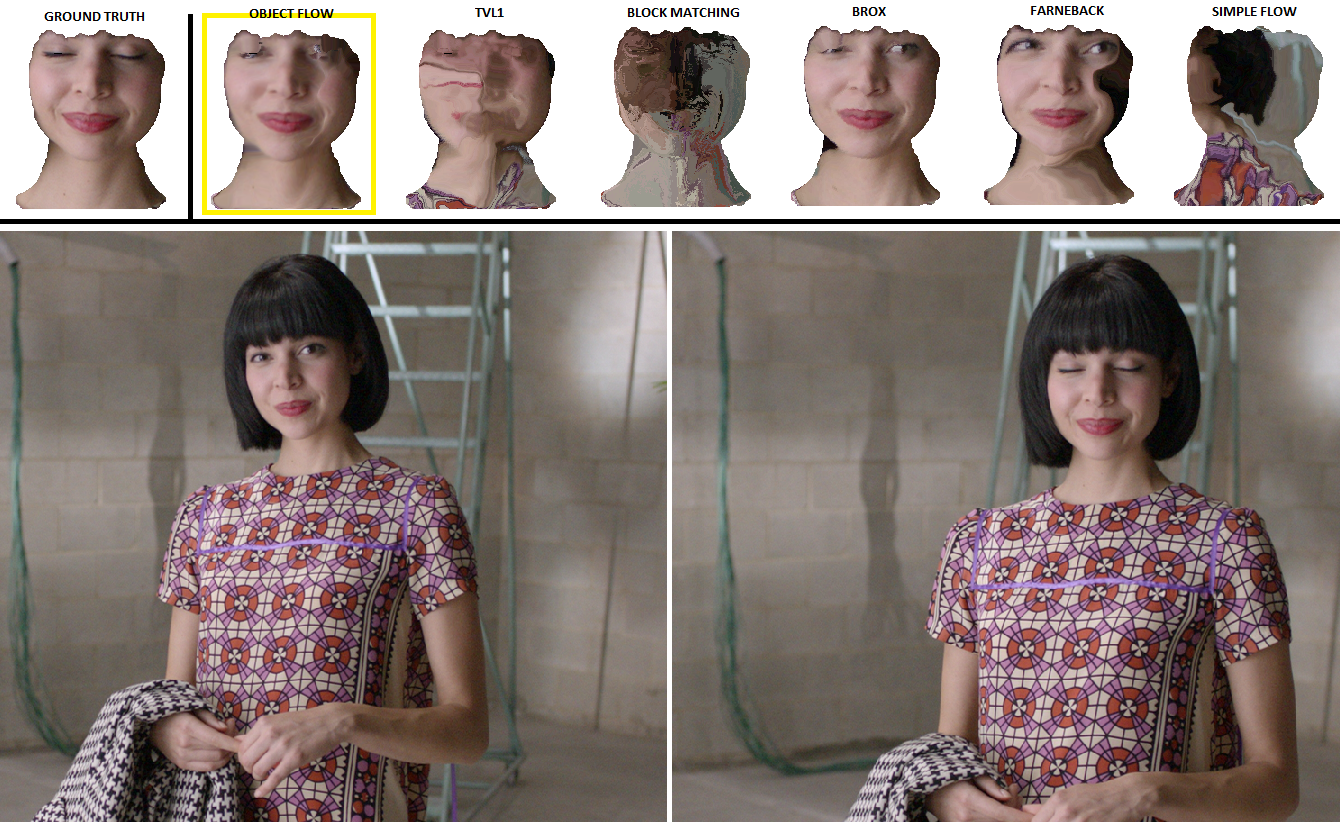
\includegraphics[width=0.375\textwidth]{../images/compare3.png}\\
  \end{tabular}
\vfill
}
%%%%%%%%%%%%%%%%%%%%%%%%%%%%%%%%%%%%%%%%%%%%%%%%%%%%%%%%%%%%%%%%%%%%%%%%%%%%%%
\headerbox{6. Applications}{name=Applications,column=2,span=2,below=results}{
\textbf{Video editing} and \textbf{Object-SfM} can use the object flow for precise and dense results.
\vfill
  \centering
  \begin{tabular}{cc}
  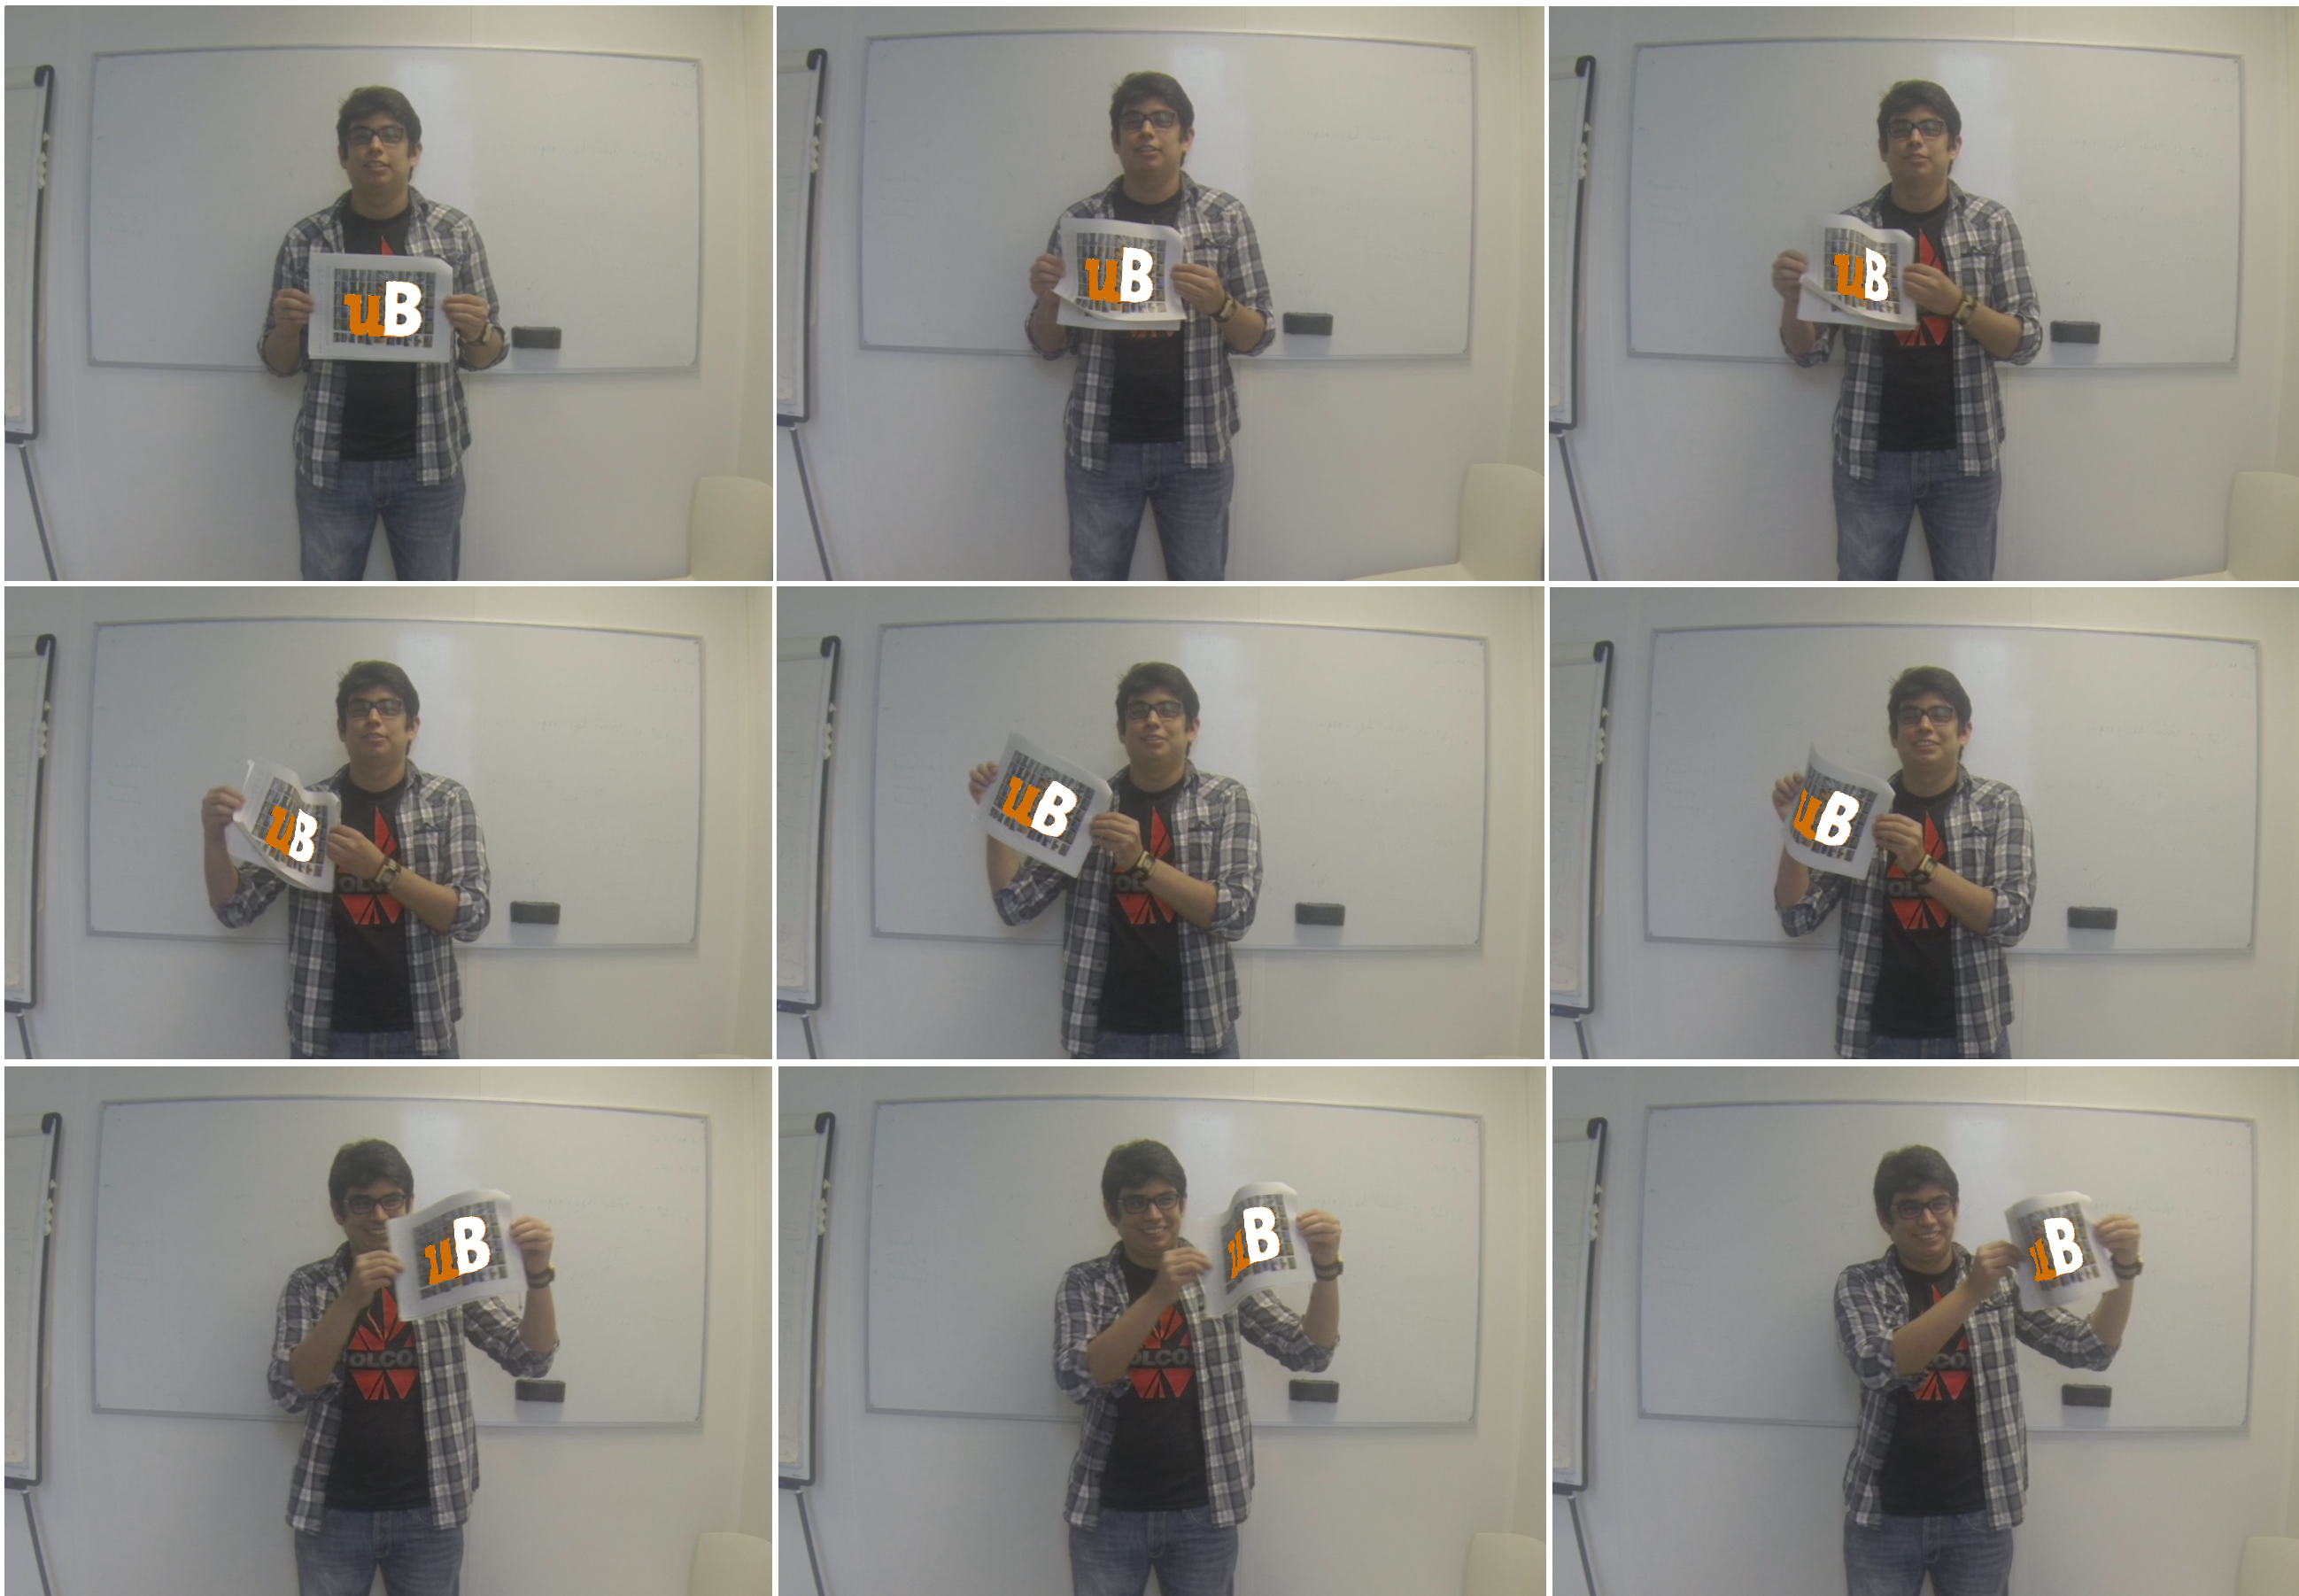
\includegraphics[height=0.266\textheight]{../images/longUB.png}&
  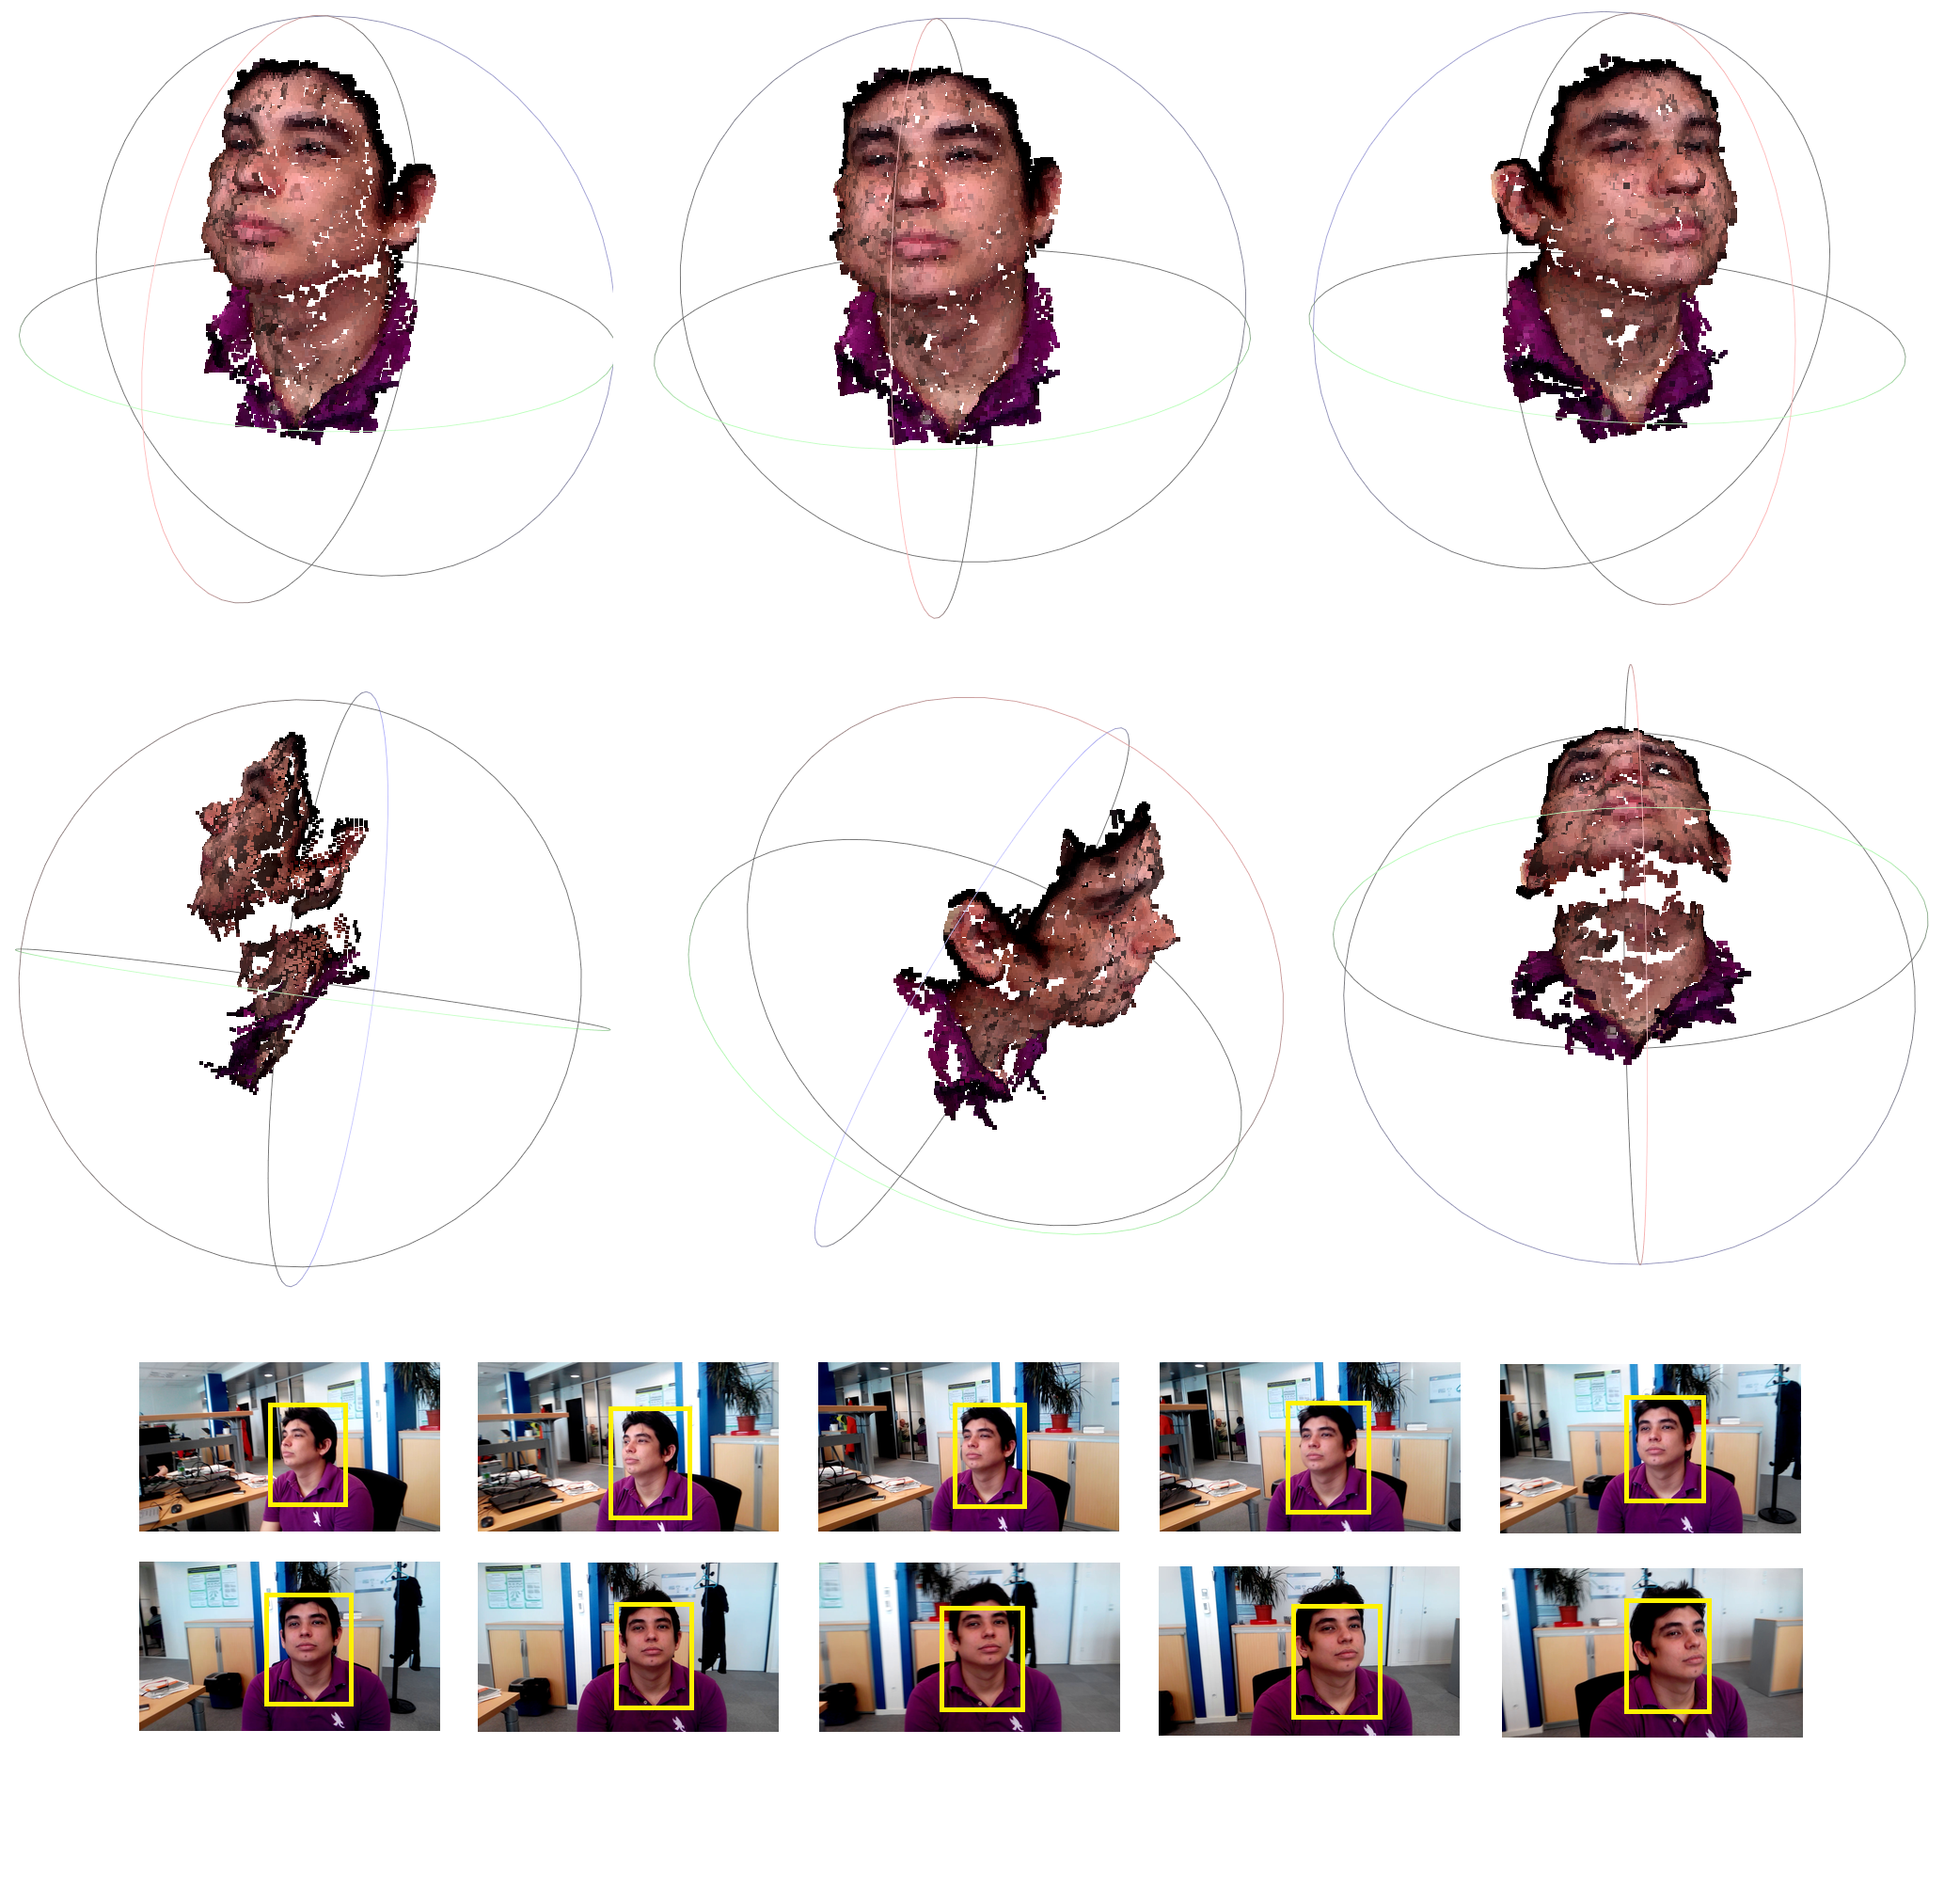
\includegraphics[height=0.266\textheight]{../images/SFM3_1.png}\\
  \end{tabular}
\vfill
}
%%%%%%%%%%%%%%%%%%%%%%%%%%%%%%%%%%%%%%%%%%%%%%%%%%%%%%%%%%%%%%%%%%%%%%%%%%%%%%
\headerbox{2. Pipeline}{name=method,column=0,below=definition}{
      \centering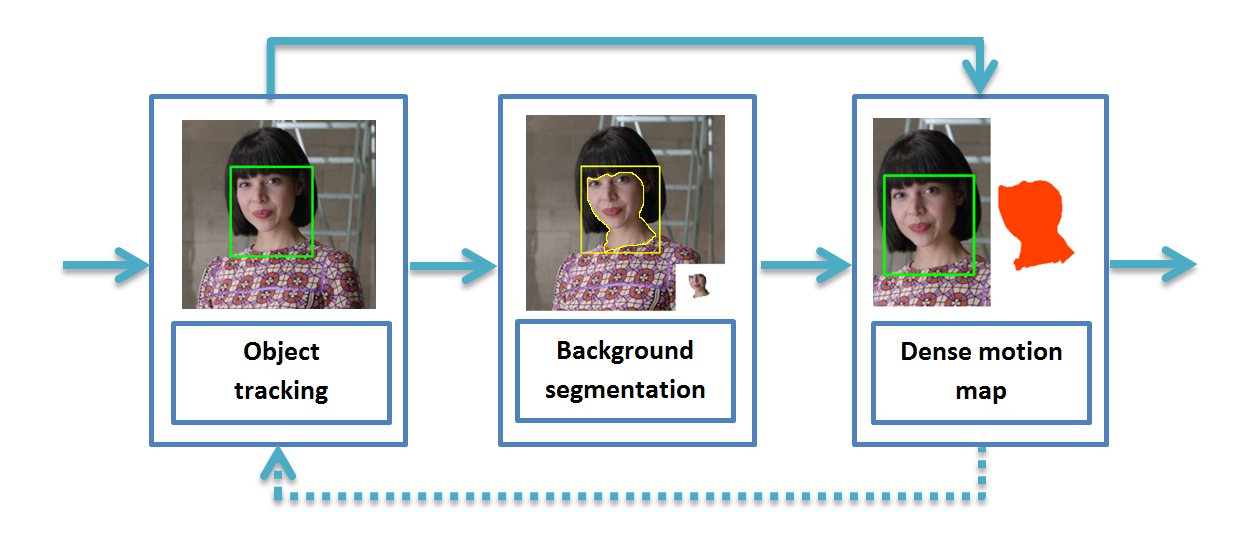
\includegraphics[width=1.00\textwidth]{../images/system.png}
      \raggedright\noindent\textbf{ Tracking. } Tracking-by-detection methods are reliable and can be improved by context information \cite{c4}. \\
      \raggedright\noindent\textbf{ Segmentation. } Video dynamics and tracker window can be used to estimate object boundaries. \\
      \raggedright\noindent\textbf{ Flow estimation. } Strong smoothness assumption is a valid prior within the estimated object boundaries \cite{c2}, and can be used 
to complete the global motion estimation given by the object tracker.
}

%%%%%%%%%%%%%%%%%%%%%%%%%%%%%%%%%%%%%%%%%%%%%%%%%%%%%%%%%%%%%%%%%%%%%%%%%%%%%%
\headerbox{4. Motion estimation}{name=motion,column=1,below=bgtrack}{
      
      \raggedright\noindent\textbf{ SimpleFlow } method \cite{c1} is modified to use segmentation masks $(S_0$ and $S_1)$ as smoothness  boundaries.

       The flow vector $(u,v)$ has to explain motion 
       in the pixel $(x_0,y_0)$ and also in its neighborhood $\mathcal{N}_{0}$, \\

      \vspace{1.5 mm}

      \centering $ E(x_0, y_0, u, v) = \sum_{(x,y) \in \mathcal{N}_{0}} w_{d}w_{c}||  I_{0}(x,y) - I_{1}(x+u,y+v) ||^2, \forall (x,y \in S_0), (x+u,y+u \in S_1)$.

      \vspace{1.5 mm}

      \centering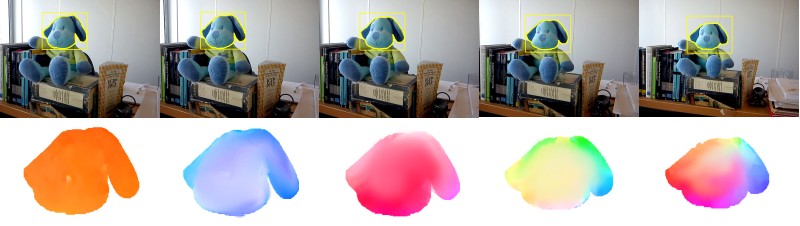
\includegraphics[width=1.00\textwidth]{../images/objectflow.png}

      \raggedright The energy is computed with a cross-bilateral filter, and the motion $(u,v)$ is found as the one that minimizes it in its local region.
       Motion is more deeply  regularized with a final Gaussian filter applied only inside these boundaries.
}

%%%%%%%%%%%%%%%%%%%%%%%%%%%%%%%%%%%%%%%%%%%%%%%%%%%%%%%%%%%%%%%%%%%%%%%%%%%%%%
  \headerbox{7. Contributions}{name=contribution,column=2,row=0,below=Applications}{
   
   Our main contributions are
   \begin{enumerate}\compresslist
   \item A method to compute superpixel matchings (The superpixel flow).
   \item A segmentation method for objects in video (Background regions tracking).
   \item A framework to combine object trackers and optical flow methods.
   \item A method to extend the Simple Flow method to use input segmentation masks.
   \item A better sampling method for tracking-by-detection methods.

   \end{enumerate}
   %\vspace{0.3em}
  }
%%%%%%%%%%%%%%%%%%%%%%%%%%%%%%%%%%%%%%%%%%%%%%%%%%%%%%%%%%%%%%%%%%%%%%%%%%%%%%
  \headerbox{8. Bibliography}{name=conclusions,column=3,row=0,below=Applications,bottomaligned=contribution}{
   
\bibliographystyle{ieee}
    \renewcommand{\section}[2]{\vskip 0.05em}
      \begin{thebibliography}{1}\itemsep=-0.01em
      \setlength{\baselineskip}{0.4em}
      
      \bibitem{c1}
      M. Tao, J. Bai, P. Kohli, and S. Paris. SimpleFlow: A Non-iterative, Sublinear Optical Flow Algorithm, {\it Eurographics '12}

      \bibitem{c2}
      S. Baker, D. Scharstein, J.P. Lewis, S. Roth, M.J. Black and R. Szeliski. A Database and Evaluation Methodology for Optical Flow, {\it IJCV '13}

      \bibitem{c3}
      Y. Boykov, M-P. Jolly. Interactive Graph Cuts for Optimal Boundary \& Region Segmentation of Objects in N-D images, {\it ICCV '13}

      \bibitem{c4}
      Y. Wu, J. Lim and M.-H. Yang. Online object tracking: A benchmark, {\it CVPR '13}

      \end{thebibliography}

   %\vspace{0.3em}
  }

\end{poster}

\end{document}
